
\section{HMI}

\subsubsection{Farger}
\begin{center}
\begin{tabular}{ | m{2.2cm} | m{2cm} |m{1.8cm} |m{5cm} |} 
\hline
	\multicolumn{4}{|c|}{\textbf{\cellcolor[HTML]{D5D5D5}Bruk av farger i HMI bilder for 3AUA Gand}} \\
\hline
	Fagre	&RGB verdi&Eksempel&Bruk\\
\hline
	Grå &213,213,213&{\cellcolor[HTML]{D5D5D5}}&Vanilg bakgrunn\\
\hline
	Hvit &255,255,255&{\cellcolor[HTML]{FFFFFF}}&Fremhevering av små\\
\hline
	Lys Grå &243,243,243&{\cellcolor[HTML]{F3F3F3}}&På indikasjon for utstyr\\
\hline
	Mørk Grå &74,74,74&{\cellcolor[HTML]{4A4A4A}}&Av indikasjon for utstyr\\
\hline
	Svart &0,0,0&{\cellcolor[HTML]{000000}}&\tiny Tekst, prosesslinjer og av grensing av prosessutstyr\normalsize\\
\hline
	Mørk blå &0,0,215&{\cellcolor[HTML]{0000D7}}&Prosessverdi\\
\hline
	Mørk grønn &0,128,0&{\cellcolor[HTML]{008000}}&\small Setpunkt og andre operatør inputs\normalsize\\
\hline
	Lys blå &187,224,227&{\cellcolor[HTML]{BBE0E3}}&ønskelige verdier\\
\hline
	Cyan &0,255,255&{\cellcolor[HTML]{00FFFF}}&Tank nivå, trend linje\\
\hline
	Brun &204,102,0&{\cellcolor[HTML]{CC6600}}&Trendlinje\\
\hline
	Rød &255,0,0&{\cellcolor[HTML]{FF0000}}&Alarm 1. prioritet\\
\hline
	Gul &255,255,0&{\cellcolor[HTML]{FFFF00}}&Alarm 2. prioritet\\
\hline
	Rød &255,102,0&{\cellcolor[HTML]{FF6600}}&Alarm 3. prioritet\\
\hline
	Magenta&255,0,255&{\cellcolor[HTML]{FF00FF}}&\small Alarm 4. prioritet for diagnostikk\\
\hline
	\small Mørk magenta&204,0,102&{\cellcolor[HTML]{E00066}}&\normalsize Trendlinje (MV)\\

\hline
\end{tabular}
\end{center}
\subsubsection{Visning av prosessverdier}

Prosessverdier med tekst skal vises med fet mørkblå skrift etterfulgt av enhet med svart skrift. For å få dette til må du lage to textfield som tilpasser hverandre:

\vskip 5pt 

\textbf{\textcolor[HTML]{0000D7}{2.3}} meter
\vskip 1cm 
Utstyr med to statuser kan vises slik:
\vskip 5pt 
\fbox{\parbox{2cm}{
	Pumpe 16:\\
	\textbf{\textcolor[HTML]{0000D7}{Startet}}
	}
}
eller
\fbox{\parbox{2cm}{
	Pumpe 16:\\
	\textbf{\textcolor[HTML]{0000D7}{Stoppet}}
	}
}
\subsubsection{Visning av alarmer}
Alarmer bør vises på en redundant måte. Det vil si at farge, form og tekst må være unke for hver alarm prioritet. 
Farger som settes av til alarm må ikke forekomme andre plasser. 
\vskip 5pt 
Eksempel:
\vskip 5pt 
\fcolorbox[HTML]{000000}{FF0000}{1} \textbf{\textcolor[HTML]{0000D7}{2.3}} meter
\vskip 5pt 
Et alarmsymbol fra Gand codesys bibliotek er satt i forbindelse med visning av en verdi for å angi alarm. Symbolet settes ti å være invisible når alarmvariablen ikke er TRUE:
\subsubsection{Bruk av symboler fra and bibilioteket}
Biblioteket finner du \href{https://rfka-my.sharepoint.com/:u:/g/personal/fred-olav_mosdal_skole_rogfk_no/EZycS5I7-ZdGjaCqIlRDeAoB0iXKpeeXCMJg4WflkLV-Sg?e=Hi4A6N}{her}. Farger som er definer kan settes inn med en \href{https://rfka-my.sharepoint.com/:u:/g/personal/fred-olav_mosdal_skole_rogfk_no/EfmBwSFs6PZCh73dTYgoGZMBGHH9Ros14TSsgv9RhuAsAA?e=EnMdNi}{visustylefil} i Codesys. 

\vskip 5pt 
\textbf{Controllerbar symbolet}
Brukes for å vise PV i forhold til SP gravisk når en ikke har behov for trend.
\vskip 5pt 
	\begin{center}
		$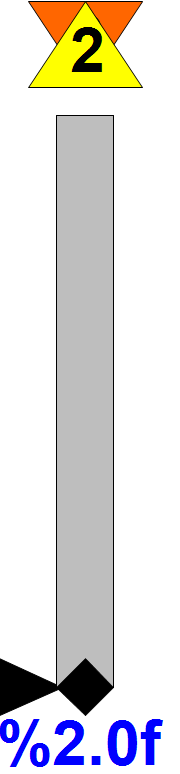
\includegraphics[height=5cm]{controllerbar.png}$\\
		Controllerbar
	\end{center}
\textbf{Loop controller settings symbolet}
Brukes for å forandre instillinger på en PID regulator. Den må kobles mot Gand.loop type variabel
\vskip 5pt 
	\begin{center}
		$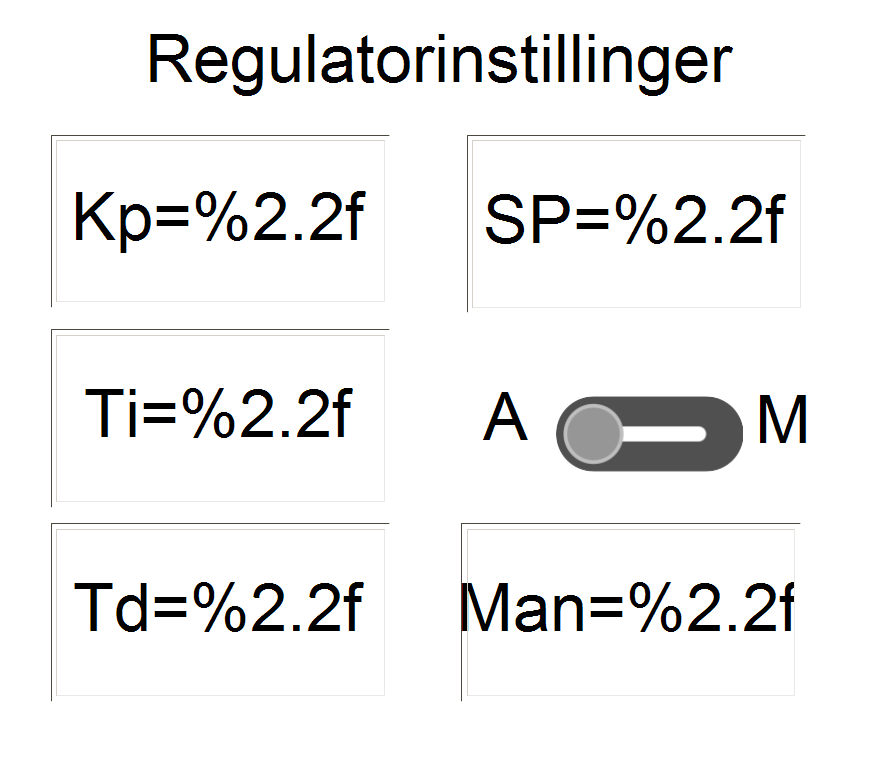
\includegraphics[height=5cm]{./Loop_Controller_settings.png}$\\
		Loop controller settings
	\end{center}
\textbf{Pump symbolet}
Brukes for å vise status på en pumpe. Er lysegrå og teksten startet vises eller er mørkegrå og stoppet vises, alt etter status på variabel som symbolet er koblet opp mot. 
\vskip 5pt 
	\begin{center}
		$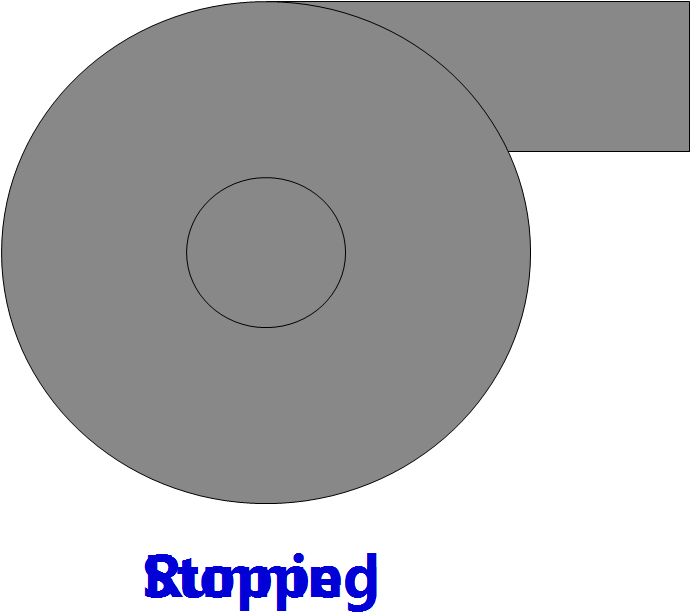
\includegraphics[height=5cm]{./HMI_pump.png}$\\
		Pump
	\end{center}
\textbf{Loop controller values symbolet}
Brukes for å vise tallverdi på PV, SP og MV over et trase. Må kobles mot Gand.loop variabel for aktuell sløyfe
\vskip 5pt 
	\begin{center}
		$
\includegraphics[height=0.5cm]{./Loop_Controller_values.png}$\\
		Loop controller values
	\end{center}
\textbf{Loop controller symbolet}
Brukes for å vise verdier og instillinger på en regulator. Må kobles mot Gand.loop variabel for aktuell sløyfe
\vskip 5pt 
	\begin{center}
		$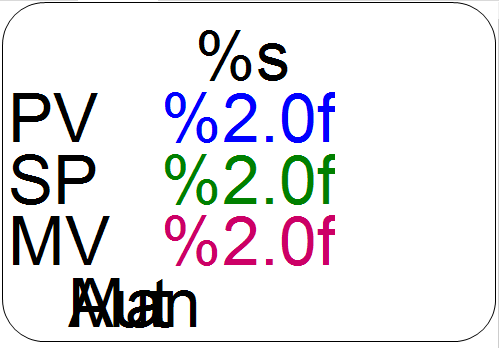
\includegraphics[height=3cm]{./Loop_Controller.png}$\\
		Loop controller
	\end{center}
\textbf{Analogvalue symbolet}
Brukes for å vise en analog verdi. Kobles mot en REAL variabel. Det må også lages en AnalogValue variabel, i denne skal en sette alle instillinger for baren. 
\vskip 5pt 
	\begin{center}
		$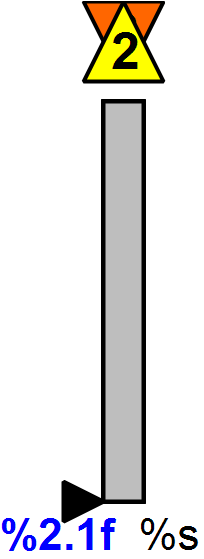
\includegraphics[height=3cm]{./analogbar.png}$\\
		AnalogValue
	\end{center}
\textbf{Control valve}
Brukes for å fremstille en reguleringsventi. Kobles mot en REAL variabel. Viser åpningen i \%
\vskip 5pt 
	\begin{center}
		$
\includegraphics[height=3cm]{./controlvalve.png}$\\
		control valve
	\end{center}
\vfil \eject

